\chapter{Biên dịch các service}
\label{Chapter2}
Phần này sẽ hướng dẫn biên dịch tất cả những service Java Spring Boot đã kể trên, bao gồm.
\begin{enumerate}
    \item Service \texttt{{authenticaion}}
    \item Service \texttt{type-service}
    \item Service \texttt{record-service}
    \item Service \texttt{notification-service}
    \item Service \texttt{service-registry}
    \item Service \texttt{api-gateway}
\end{enumerate}

\section{Tạo file JAR}
Từ thư mục gốc \texttt{salesync} của mã nguồn. Truy cập vào thư mục \texttt{back-end} và truy cập thư mục con tương ứng với tên của service cần biên dịch.
Tiến hành chạy lệnh \texttt{mvn clean install} để Apache Maven biên dịch mã nguồn Java thành file JAR và lưu vào thư mục con target tại \\
\texttt{salesync/back-end/service-cần-biên-dịch/target}.

Nếu thành công, kết quả trả về sẽ có dạng như Hình ~\ref{fig:maven_build_successfully}.

\begin{figure}
    \centering
    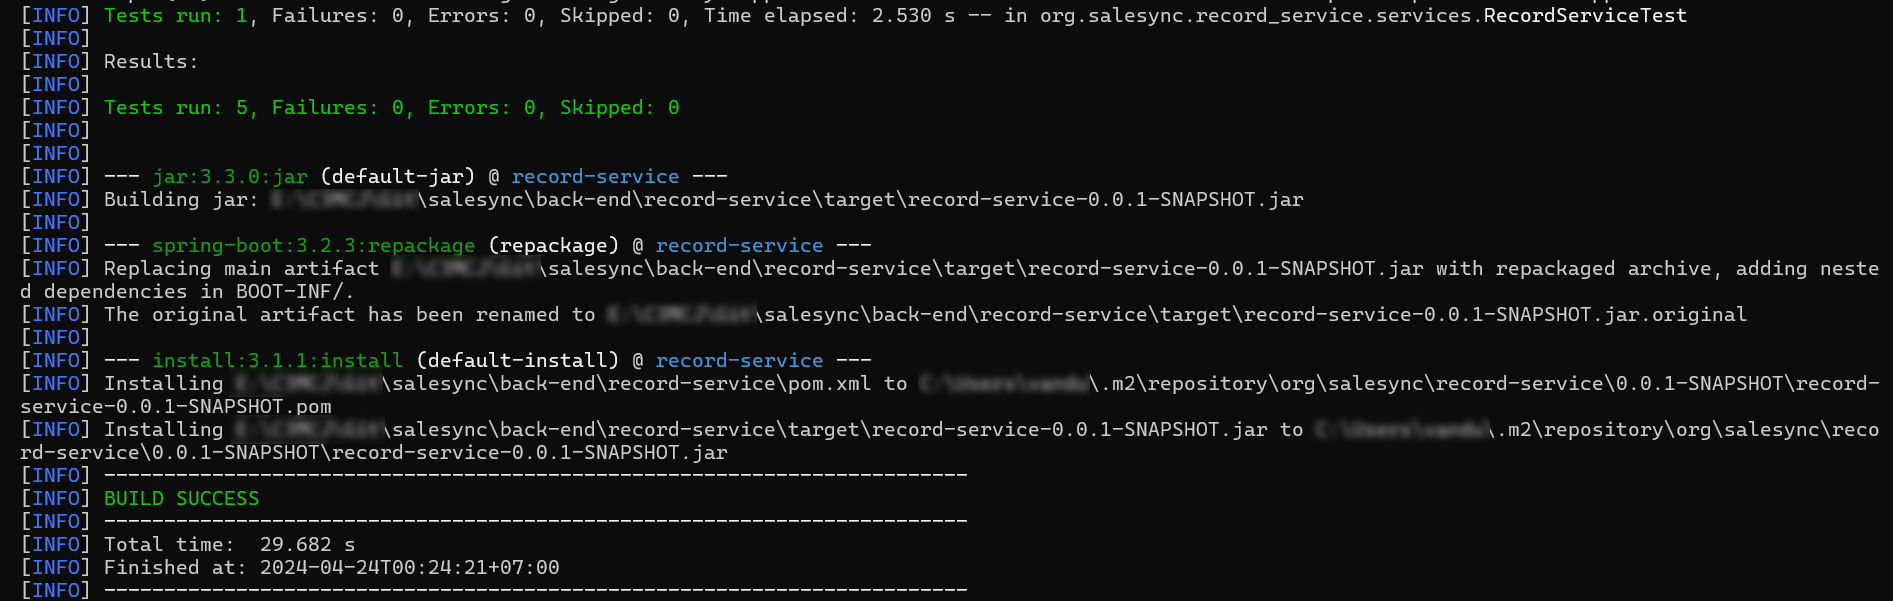
\includegraphics[width=1\linewidth]{maven_build_successfully.png}
    \caption{Kết quả trả về khi tạo file thành công}
    \label{fig:maven_build_successfully}
\end{figure}

\section{Lưu lại file JAR}
Tạo thư mục \texttt{artifacts} và lưu file  JAR vừa tạo tại \\
\texttt{salesync/back-end/service-cần-biên-dịch/artifacts}

\section{Lặp lại với các service khác}
Thực hiện những bước tương tự với các service khác, kết quả đạt được bao gồm $6$ file JAR khác nhau tương ứng với $6$ service đã liệt kê. Đây cũng là sản phẩm cuối cùng của quy trình biên dịch các Service.